


\tikzset{every picture/.style={line width=0.75pt}} %set default line width to 0.75pt        


\def \xOne {12}
\def \xTwo {522}
\def \yOne {165}
\def \yTwo {195}
\def \yOneDelta {40}
\def \yTwoDelta {35}
\def \yTwoShift {5}

\def \hcboxXOne{20}
\def \hcboxXTwo{110}
\def \hcboxYOne{25}
\def \hcboxYTwo{50}
\def \hcboxXShift{100}

\def \dsXOne{60}
\def \dsXTwo{190}
\def \dsYOne{130}
\def \dsYTwo{155}
\def \dsXShift{270}

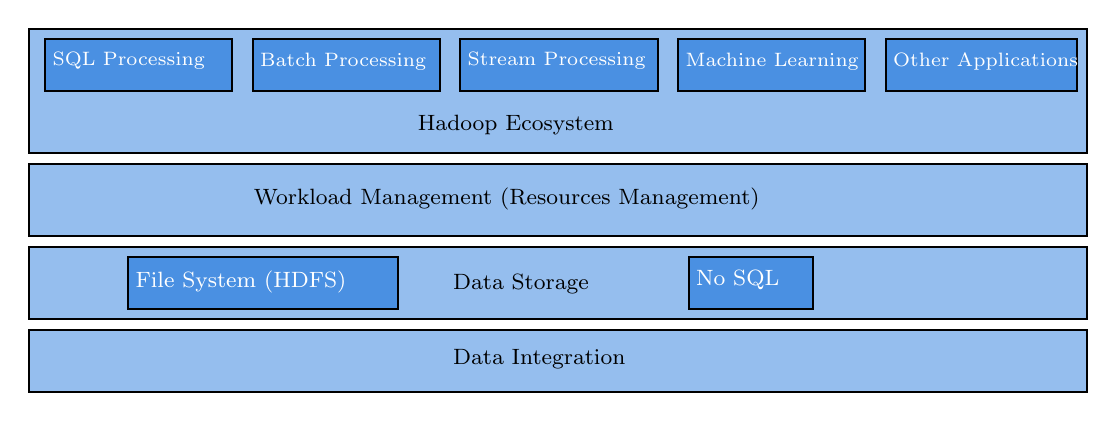
\begin{tikzpicture}[x=0.75pt,y=0.75pt,yscale=-1,xscale=1]

	
	%Shape: Rectangle [id:dp9526398227547324] 
	\draw [fill={rgb, 255:red, 74; green, 144; blue, 226 }  ,fill opacity=0.59 ] (\xOne,\yOne) -- (\xTwo,\yOne) -- (\xTwo,\yTwo) -- (\xOne,\yTwo) -- cycle ;
	%Shape: Rectangle [id:dp34591779607428674] 
	\draw  [fill={rgb, 255:red, 74; green, 144; blue, 226 }  ,fill opacity=0.59 ] (\xOne,\yOne-\yOneDelta) -- (\xTwo,\yOne-\yOneDelta) -- (\xTwo,\yTwo-\yTwoDelta) -- (\xOne,\yTwo-\yTwoDelta) -- cycle ;

	%Shape: Rectangle [id:dp45758690857887285] 
	\draw [fill={rgb, 255:red, 74; green, 144; blue, 226 }  ,fill opacity=0.59 ] (\xOne,\yOne-\yOneDelta*2) -- (\xTwo,\yOne-\yOneDelta*2) -- (\xTwo,\yTwo-\yTwoDelta*2 - \yTwoShift) -- (\xOne,\yTwo-\yTwoDelta*2 - \yTwoShift) -- cycle ;
	%Shape: Rectangle [id:dp7537784714823494] 
	\draw [fill={rgb, 255:red, 74; green, 144; blue, 226 }  ,fill opacity=0.59 ] (\xOne,\yOne-\yOneDelta*3-25) -- (\xTwo,\yOne-\yOneDelta*3-25) -- (\xTwo,\yTwo-\yTwoDelta*3 -\yTwoShift*2) -- (\xOne,\yTwo-\yTwoDelta*3 -\yTwoShift*2) -- cycle ;
	
	
	%Rounded Rect [id:dp9146242593539052] 
	\draw  [fill={rgb, 255:red, 74; green, 144; blue, 226 }  ,fill opacity=1 ] (\dsXOne,\dsYOne) -- (\dsXTwo,\dsYOne) -- (\dsXTwo,\dsYTwo) -- (\dsXOne,\dsYTwo) -- cycle ;
	%Rounded Rect [id:dp07383423201361416] 
	\draw  [fill={rgb, 255:red, 74; green, 144; blue, 226 }  ,fill opacity=1 ] (\dsXOne+\dsXShift,\dsYOne) -- (\dsXTwo-70+\dsXShift,\dsYOne) -- (\dsXTwo+\dsXShift-70,\dsYTwo) -- (\dsXOne+\dsXShift,\dsYTwo) -- cycle ;
	
	
	
	
	%Rounded Rect [id:dp8181874793090042] 
	\draw  [fill={rgb, 255:red, 74; green, 144; blue, 226 }  ,fill opacity=1 ] (\hcboxXOne,\hcboxYOne) -- (\hcboxXTwo,\hcboxYOne) -- (\hcboxXTwo,\hcboxYTwo) -- (\hcboxXOne,\hcboxYTwo) -- cycle ;
	%Rounded Rect [id:dp9716087561496145] 
	\draw  [fill={rgb, 255:red, 74; green, 144; blue, 226 }  ,fill opacity=1 ] (\hcboxXOne+\hcboxXShift,\hcboxYOne) -- (\hcboxXTwo+\hcboxXShift,\hcboxYOne) -- (\hcboxXTwo+\hcboxXShift,\hcboxYTwo) -- (\hcboxXOne+\hcboxXShift,\hcboxYTwo) -- cycle ;
	%Rounded Rect [id:dp6064393858129398] 
	\draw  [fill={rgb, 255:red, 74; green, 144; blue, 226 }  ,fill opacity=1 ] (\hcboxXOne+\hcboxXShift*2,\hcboxYOne) -- (\hcboxXTwo+\hcboxXShift*2+5,\hcboxYOne) -- (\hcboxXTwo+\hcboxXShift*2+5,\hcboxYTwo) -- (\hcboxXOne+\hcboxXShift*2,\hcboxYTwo) -- cycle ;
	%Rounded Rect [id:dp9339323209047331] 
	\draw  [fill={rgb, 255:red, 74; green, 144; blue, 226 }  ,fill opacity=1 ] (\hcboxXOne+\hcboxXShift*3+5,\hcboxYOne) -- (\hcboxXTwo+\hcboxXShift*3+5,\hcboxYOne) -- (\hcboxXTwo+\hcboxXShift*3+5,\hcboxYTwo) -- (\hcboxXOne+\hcboxXShift*3+5,\hcboxYTwo) -- cycle ;
	%Rounded Rect [id:dp5657335982682512] 
	\draw  [fill={rgb, 255:red, 74; green, 144; blue, 226 }  ,fill opacity=1 ] (\hcboxXOne+\hcboxXShift*4+5,\hcboxYOne) -- (\hcboxXTwo+\hcboxXShift*4+7,\hcboxYOne) -- (\hcboxXTwo+\hcboxXShift*4+7,\hcboxYTwo) -- (\hcboxXOne+\hcboxXShift*4+5,\hcboxYTwo) -- cycle ;

	% Text Node
	\draw (215,173) node [anchor=north west][inner sep=0.75pt]  [font=\footnotesize] [align=left] {Data Integration};
	% Text Node
	\draw (\dsXOne+2,\dsYOne+5) node [anchor=north west][inner sep=0.75pt]  [font=\footnotesize,color={rgb, 255:red, 255; green, 255; blue, 255 }  ,opacity=1 ] [align=left] {File System (HDFS)};
	% Text Node
	\draw (\dsXOne+\dsXShift+2,\dsYOne+5) node [anchor=north west][inner sep=0.75pt]  [font=\footnotesize,color={rgb, 255:red, 255; green, 255; blue, 255 }  ,opacity=1 ] [align=left] {No SQL};

	% Text Node
	\draw (215,137) node [anchor=north west][inner sep=0.75pt]  [font=\footnotesize] [align=left] {Data Storage};
	% Text Node
	\draw (119,95) node [anchor=north west][inner sep=0.75pt]  [font=\footnotesize] [align=left] {Workload Management (Resources Management)};
	% Text Node
	\draw (198,60) node [anchor=north west][inner sep=0.75pt]  [font=\footnotesize] [align=left] {Hadoop Ecosystem};
	
	% Text Node
	\draw (\hcboxXOne +2 ,\hcboxYOne +5) node [anchor=north west][inner sep=0.75pt]  [font={\scriptsize },color={rgb, 255:red, 255; green, 255; blue, 255 }  ,opacity=1 ] [align=left] {SQL Processing};
	% Text Node
	\draw (\hcboxXOne +2+\hcboxXShift,\hcboxYOne +5) node [anchor=north west][inner sep=0.75pt]  [font=\scriptsize,color={rgb, 255:red, 255; green, 255; blue, 255 }  ,opacity=1 ] [align=left] {Batch Processing};
	% Text Node
	\draw (\hcboxXOne +2+\hcboxXShift*2,\hcboxYOne +5) node [anchor=north west][inner sep=0.75pt]  [font=\scriptsize,color={rgb, 255:red, 255; green, 255; blue, 255 }  ,opacity=1 ] [align=left] {Stream Processing};
	% Text Node
	\draw (\hcboxXOne +7+\hcboxXShift*3,\hcboxYOne +5) node [anchor=north west][inner sep=0.75pt]  [font=\scriptsize,color={rgb, 255:red, 255; green, 255; blue, 255 }  ,opacity=1 ] [align=left] {Machine Learning};
	% Text Node
	\draw (\hcboxXOne +7+\hcboxXShift*4,\hcboxYOne +5) node [anchor=north west][inner sep=0.75pt]  [font=\scriptsize,color={rgb, 255:red, 255; green, 255; blue, 255 }  ,opacity=1 ] [align=left] {Other Applications};
	
	
\end{tikzpicture}
%%%%%%%%%%%%%%%%%%%%%%%%%%%%%%%%%%%%%%%%%%%%%%%%%%%%%%%%%%%%%%%%%%%%%%%%%%%
%%% Local Variables:
%%% mode: latex
%%% TeX-master: "../../main.tex"
% !TeX root = ../../main.tex
%%% TeX-engine: xetex
%%% End:
